\section{The final PHASE-TTC system}
\label{sec:train40}

\subsection{Deployed model composition}

PHASE-TTC deploys a causal chain of nine fitted components derived from the V16 PHASE-ONLY family: four modality-specific producers, two PAIR heads, two context refiners, and one fusion head. RGB and events each use an A5 baseline producer and a coarse-to-fine C2F producer. The PAIR readouts extract phase features from their A5 representations, after which the context refiners incorporate temporal history. The fusion head anchors its correction on the refined RGB estimate. Figure~\ref{fig:deployed-architecture} traces this path; the five auxiliary rotations serve training only. \evidence{M22,M23}

\begin{figure}[htbp]
  \centering
  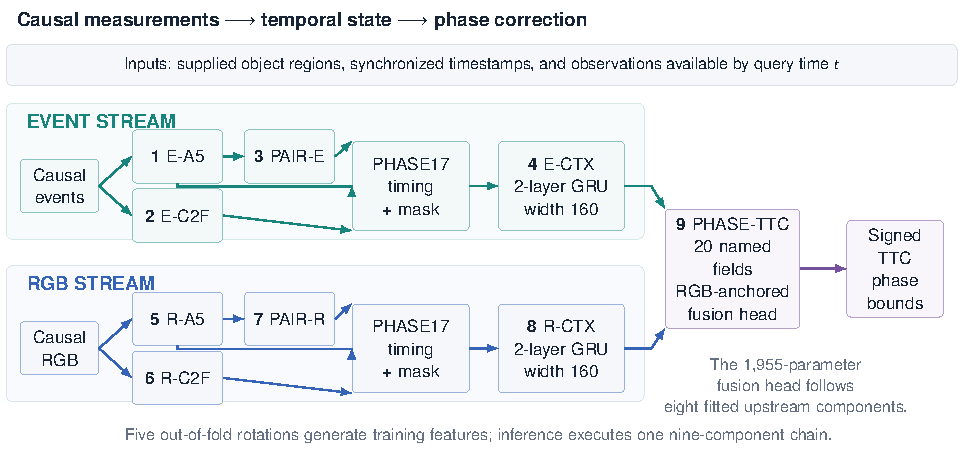
\includegraphics[width=\linewidth]{figures/rev_architecture.pdf}
  \caption{\textbf{Causal nine-component inference graph.} Supplied object regions feed parallel RGB and event producers, PAIR heads, and temporal refiners. Twenty named fields enter the final RGB-anchored fusion head. \evidence{M03,M22,M23}}
  \label{fig:deployed-architecture}
\end{figure}

Final fitting uses 88,744 TRAIN40 queries from forty sequences. The former P, H, and V groups all contribute to this refit, so their earlier scores characterize development rather than independent validation of the deployed chain. Each producer receives 49,932 updates, equivalent to eighteen epochs at effective batch size 32. The event producers carry forward the earlier TRAIN40 weights; RGB training resumes to the same endpoint. \evidence{L43}

\subsection{Object coordinates and causal history}

Each query includes supplied object coordinates. A common spatial frame covers both endpoint regions and preserves apparent scale change, which independent tight crops can erase. The evaluated system therefore assumes external localization. \evidence{M03}

Both branches use observations available by query time \(t\), with up to 650\,ms of causal history. Runtime begins at its declared measurement boundary and ends when the host receives the TTC output at \(t+L\). Figure~\ref{fig:causal-history} separates the sensing interval from response time; its observation marks are schematic. \evidence{M22,L43,L44}

\begin{figure}[H]
  \centering
  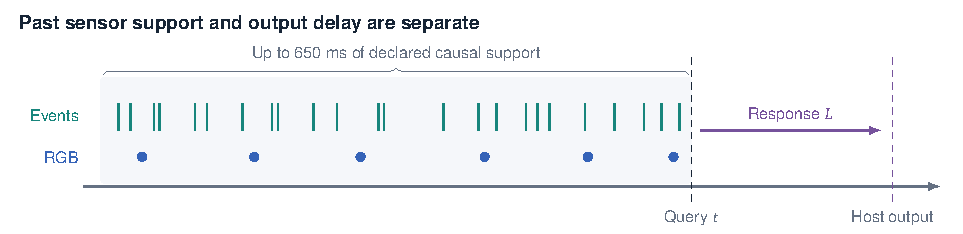
\includegraphics[width=\linewidth]{figures/rev_history.pdf}
  \caption{\textbf{Causal support and response-time boundaries.} RGB and event observations precede query time \(t\). The latency clock spans the declared runtime boundary to the complete host TTC output at \(t+L\).}
  \label{fig:causal-history}
\end{figure}

\subsection{Compact fusion interface}

Each context refiner is represented for final fusion by a constructed 170-coordinate block. Coordinates 0--159 are its learned hidden state. Coordinates 160--169 are an explicit interface containing, in order, one raw location, one emitted phase, three expert phases, four current timing values, and one valid-history count divided by eight. Concatenating the RGB block followed by the event block gives the 340-coordinate container
\begin{equation}
  \mathbf{s}=\left[\mathbf{s}_{R}^{170};\mathbf{s}_{E}^{170}\right]\in\mathbb{R}^{340}.
\end{equation}
Fusion reads \(\mathbf{s}_{160:170}\) and \(\mathbf{s}_{330:340}\), yielding twenty named phase, timing, and support inputs while the 160-dimensional hidden states remain within their modality branches. Within each ten-coordinate block, the first five phase coordinates are divided by \(0.03\); timing and support keep their native scaling. The shared interface aligns quantities with consistent meanings across the separately fitted refiners. \evidence{M22}

The selected vector passes through
\begin{equation}
  20\rightarrow 32\;[\mathrm{LayerNorm},\mathrm{SiLU}]
  \rightarrow 32\;[\mathrm{LayerNorm},\mathrm{SiLU}]
  \rightarrow 3.
\end{equation}
Zero initialization of the last affine layer makes the initial fusion output equal to the RGB anchor. If \(c_0,c_1,c_2\) are the three head outputs, \(\ell_R\) is the RGB raw-location anchor, and \(\mathbf{w}_R\) is the separately supplied pair of RGB width logits, the deployed computation is
\begin{align}
  \ell_F &= \ell_R + 0.03c_0, \\
  \boldsymbol{\sigma}_F &= 0.03\,\operatorname{softplus}\!\left(\mathbf{w}_R+[c_1,c_2]\right), \\
  \widehat{\mathrm{TTC}} &= \operatorname{phase\_to\_ttc}(\ell_F), \\
  q_{10}^{\phi} &= \operatorname{clip}(\ell_F-\sigma_{F,0},\,\phi_{\min},\phi_{\max}), \\
  q_{90}^{\phi} &= \operatorname{clip}(\ell_F+\sigma_{F,1},\,\phi_{\min},\phi_{\max}).
\end{align}
The native bounds are \(\phi_{\min}=-\log 2+10^{-6}\) and \(\phi_{\max}=8\). For the point prediction, the inverse map clamps \(\ell_F\) to these bounds, computes \(q=-\operatorname{expm1}(-\phi)/0.1\), and emits \(\operatorname{sgn}_{+}(q)/\max(|q|,1/60)\) seconds, where \(\operatorname{sgn}_{+}(0)=1\). Thus the emitted magnitude is at most 60\,s and zero phase maps to \(+60\)\,s. The reported point phase is recomputed from this finite TTC; the learned-width phase-interval endpoints are clamped separately. Saturation is a numerical convention, not a measured 60-second collision time or a calibration result. \evidence{M22,R02}

The compact fusion head contains 1,955 trainable parameters: \(672+64+1{,}056+64+99\) across three affine layers and two LayerNorms. Figure~\ref{fig:fusion-interface} summarizes the slicing and anchored output map. \evidence{M22}

\begin{figure}[htbp]
  \centering
  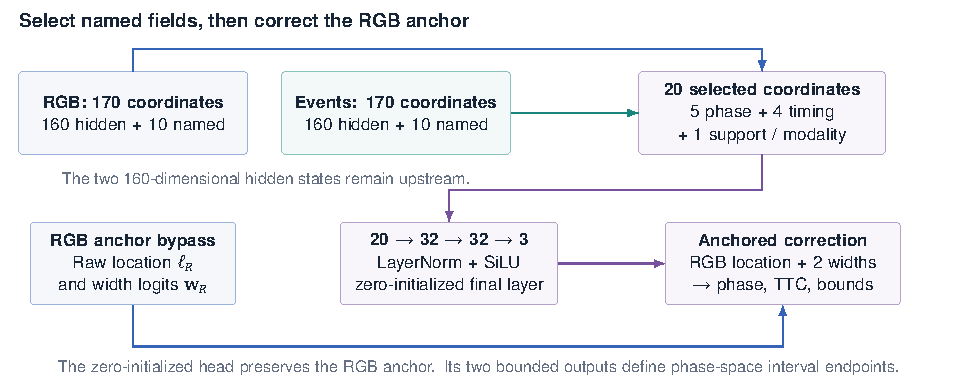
\includegraphics[width=\linewidth]{figures/rev_fusion.pdf}
  \caption{\textbf{Named-feature fusion interface.} Twenty phase, timing, and support coordinates are selected from the 340-value container. The RGB anchor and width logits follow a separate bypass into the three-output correction head. \evidence{M22}}
  \label{fig:fusion-interface}
\end{figure}

\subsection{Submission coverage and benchmark status}

The official submission contains finite predictions without fallback for 6,762 query tokens across twelve sequences: 5,805 physical queries and 957 aliases. Aliases identify repeated physical queries and do not represent additional inference work. \evidence{L44}

Section~\ref{sec:official} reports the official test result for this V16-derived PHASE-ONLY graph. The later V18 controls evaluate a different configuration. \evidence{B01,B02,L44}
